\section*{CHƯƠNG 4. TRIỂN KHAI VÀ THỬ NGHIỆM}
    \addcontentsline{toc}{section}{\numberline{} CHƯƠNG 4. MÔ PHỎNG VÀ KẾT QUẢ}
\setcounter{section}{4}
    \setcounter{subsection}{0}
        \setcounter{figure}{0}
            \setcounter{table}{0}
                \setcounter{equation}{0}

%--------------------------------------------------------%

\subsection{Quy trình triển khai}

\hspace{0.8cm} Ở chương này em trình bày chi tiết quá trình triển khai, xây dựng sản phẩm sử dụng các công nghệ đã lựa chọn ở Chương 2 và dựa trên thiết kế chi tiết đã nêu ra ở Chương 3.

Nội dung gồm quy trình triển khai, mô tả đầu ra sản phẩm,
kiểm thử và chạy với dữ liệu mô phỏng, lắp ráp và kiểm thử tại hiện trường.

\subsubsection{Mạch phần cứng thiết bị đọc màn hình}

\textbf{a. Vẽ mạch PCB từ sơ đồ nguyên lý}

Từ sơ đồ nguyên lý đã đã nêu ở Chương 3, tiến hành vẽ mạch PCB trên Altium:

\begin{figure}[!ht]
    \centering
    \includegraphics[width=0.8\linewidth]{Figures/PCB_top-down.png}
   
    \caption{Mạch PCB - Mặt trên}
    \label{fig:PCB_top-down}
\end{figure}

\begin{figure}[!ht]
    \centering
    \includegraphics[width=0.4\linewidth]{Figures/PCB_side-view.png}
    \hspace{0.1\textwidth}
    \includegraphics[width=0.4\textwidth]{Figures/PCB_bottom-up.png}
    \caption{Mạch PCB - Mặt ngang và mặt dưới}
    \label{fig:PCB_side-view-and-bottom-up}
\end{figure}

\FloatBarrier
\textbf{ b. In và hàn mạch thực tế}
\begin{figure}[!ht]
    \centering
    \includegraphics[width=0.8\linewidth]{Figures/Device_product-top-down.jpg}
    \caption{Sản phẩm thiết bị đọc ghi màn hình cột bơm: mặt trên}
    \label{fig:Device_product-top-down}
\end{figure}

\begin{figure}[!ht]
    \centering
    \includegraphics[width=0.45\linewidth]{Figures/Device_product-bottom-view.jpg}
    \hspace{0.02\textwidth}
    \includegraphics[width=0.45\textwidth]{Figures/Device_product-side-view.jpg}
    \caption{Sản phẩm thiết bị đọc ghi màn hình cột bơm: mặt ngang và dưới}
    \label{fig:device_product}
\end{figure}


\subsubsection{Firmware thiết bị đọc màn hình}

Môi trường/ công cụ phát triển để lập trình cho STM32: STM32CubeIDE.

\textbf{Setup các cổng IO}

\begin{figure}[!ht]
    \centering
    \includegraphics[width=1.0\linewidth]{Figures/Device_stm32-io-config.png}
    \caption{Triển khai: cấu hình các chân trong STM32CubeIDE}
    \label{fig:Device_stm32-io-config}
\end{figure}

Các ngoại vi được sử dụng bao gồm:
\begin{itemize}
    \item SPI1: Kết nối với module W5500, giao tiếp Ethernet.
    \item SPI2: Kết nối với CPLD, nhận dữ liệu màn hình dạng byte data.
    \item USART2: Sử dụng để debug (kết nối với máy tính và gửi thông báo lên màn hình terminal)
    \item Các cổng IO khác:
    \begin{itemize}
        \item PB12 và PB13: điều khiển relay 1 và 2.
        \item PA1, PA2 và PA3: các đèn báo led.
        \item PA9: CPLD Enable
        \item PC9: Frame Stop - Ngắt GPIO đầu vào báo kết thúc 1 frame 
    \end{itemize}
\end{itemize}

\FloatBarrier
\textbf{Triển khai firmware}

 \hspace{0.8cm} Về tổ chức các thư mục, tại thư mục \texttt{core/Src} tổ chức thành 4 thư mục lớn chứa 4 modules được nêu trong phần Kiến trúc triển khai firmware (xem hình minh họa ở chương trước) là: \texttt{capture\_driver}, \texttt{device\_driver}, \texttt{internet} và \texttt{fota}

 Các thuật toán quan trọng bao gồm:

 \begin{itemize}
    \item Khởi tạo và kết nối với phần mềm Device Service
    \item Xử lý ngắt SPI1: Nhận yêu cầu từ Device Service
    \item Xử lý ngắt SPI2: Nhận SPI byte từ CPLD
    \item Xử lý ngắt báo Frame Stop: Báo kết thúc 1 screen frame và tiến hành lưu frame
 \end{itemize}


\begin{figure}[!ht]
    \centering
    \includegraphics[width=1.0\linewidth]{Figures/flowcharts-Device_Receive-screen-frame.png}
    \caption{Thuật toán xử lý ngắt nhận dữ liệu màn hình}
    \label{fig:flowcharts-Device_Receive-screen-frame}
\end{figure}


\begin{figure}[!ht]
    \centering
    \includegraphics[width=1.0\linewidth]{Figures/flowcharts-Device_handle-DS-req.png}
    \caption{Thuật toán xử lý ngắt nhận dữ yêu cầu Device Service}
    \label{fig:flowcharts-Device_handle-DS-req}
\end{figure}
 

\begin{figure}[!ht]
    \centering
    \includegraphics[width=1.0\linewidth]{Figures/flowcharts-Device_Main loop.png}
    \caption{Thuật toán cho chương trình chính}
    \label{fig:flowcharts-Device_Main loop}
\end{figure}

\FloatBarrier

Cấu trúc gói tin giao tiếp giữa Thiết bị đọc ghi màn hình (Device) và Phần mềm giải mã (Device Service) được nêu trong bảng \ref{tab:device-packet_structure}

\begin{table}[h!]
\centering
\begin{tabular}{|c|c|c|p{7cm}|}
\hline
\textbf{Trường} & \textbf{Kích thước} & \textbf{Offset} & \textbf{Mô tả} \\
\hline
Packet Length & 2 bytes & 0–1 & Tổng chiều dài gói tin trừ đi 12 byte đầu (độ dài Payload). \\
\hline
Device MAC & 6 bytes & 2–7 & Địa chỉ MAC của thiết bị đọc ghi màn hình \\
\hline
CMD & 1 byte & 8 & Loại lệnh (command) được gửi (xem bảng \ref{tab:cmd_list}). \\
\hline
Reserved & 3 bytes & 9–11 & 3 byte dự phòng, chưa sử dụng. \\
\hline
Payload & Tùy loại CMD & 12 trở đi & Dữ liệu phụ thuộc vào từng loại CMD, ví dụ frame màn hình, trạng thái relay, v.v. \\
\hline
\end{tabular}
\caption{Cấu trúc gói tin giữa Device và Device Service}
\label{tab:device-packet_structure}
\end{table}


Các loại Command (CMD) để giao tiếp với Thiết bị:

\begin{longtable}{|c|l|p{6cm}|}
\hline
\textbf{CMD} & \textbf{Tên} & \textbf{Mô tả} \\
\hline
\endfirsthead



0x01 & CMD\_HANDSHAKE & CMD Handshake, dùng để gửi từ `Device` đến `Device Service`. \\
\hline
0x02 & CMD\_REPORT\_RAWDATA & CMD gửi frame màn hình, dùng để stream screen frame từ `Device` đến `Device Service`. \\
\hline
0x03 & CMD\_REPORT\_RELAY & CMD gửi trạng thái relay từ `Device` đến `Device Service`. \\
\hline
0x04 & CMD\_SET\_RELAY & CMD yêu cầu đặt trạng thái relay từ `Device Service` đến `Device`. \\
\hline
0x05 & CMD\_TIME\_SYNC & CMD yêu cầu đồng bộ thời gian từ `Device Service` đến `Device`. \\
\hline
0x06 & CMD\_PING & CMD ping kiểm tra kết nối từ `Device Service` đến `Device`. \\
\hline
0x07 & CMD\_OTA\_START & CMD yêu cầu bắt đầu OTA từ `Device Service` đến `Device`. \\
\hline
0x08 & CMD\_OTA\_SEND\_FILE & CMD yêu cầu gửi file OTA từ `Device Service` đến `Device`. \\
\hline
0x09 & CMD\_OTA\_ACTIVE\_FIRM & CMD yêu cầu kích hoạt firmware mới từ `Device Service` đến Device`. \\
\hline
0x0A & CMD\_OTA\_OTA\_RESP & CMD phản hồi OTA từ `Device` đến `Device Service`. \\
\hline

\caption{Danh sách các loại CMD trong enum Cmd\_t}
\label{tab:cmd_list}
\end{longtable}



\subsubsection{Phần mềm giải mã Device Service}

Chuẩn bị môi trường:

\begin{itemize}
    \item Môi trường phát triển: Visual Studio.
    \item Ngôn ngữ: C++.
    \item Loại dự án: Win32 API C++.
    \item Các thư viện được sử dụng: Boost, 
\end{itemize}


Các bước triển khai:

Bước 1: Tạo 1 Win32 Application Project

\begin{figure}[!ht]
     \centering
    \includegraphics[width=1\linewidth]{Figures/DeviceService-create-project.png}
    \caption{:Tạo C++ Win32 Project trên Visual Studio}
    \label{fig:Tạo C++ Win32 Project trên Visual Studio}
\end{figure}

Bước 2: Triển khai chế độ chạy cho phần mềm.

Triển khai để khi phần mềm được khởi chạy sẽ:
\begin{itemize}
    \item Tạo 1 mutex riêng có tên cố định trên Window, đảm bảo dù nhấn mở phần mềm nhiều lần thì vẫn sẽ chỉ có 1 Instance của App đang chạy.
    \item Phần mềm không có giao diện, sẽ là 1 tác vụ chạy ngầm trên Window (Window Service).

\end{itemize}

Bước 3: Viết các khối triển khai.

Các khối triển khai tuân theo thiết kế ở hình \ref{fig:DeviceService_implementation-block}

Phần này nêu chi tiết những thuật toán quan trọng cho các khối

\textbf{Thuật toán bộ giải mã và phát hiện trạng thái máy} 

Khối thực hiện: Logger.

Một `log` (lượt bơm) được chốt sau khi giá trị màn hình (số lít và giá tiền) dừng tăng trong 5 giây, hoặc cột đang bơm thì dừng và reset màn hình.

Một `log` cũng có thể dùng để lưu màn hình hiển thị giá trị preset (đặt trước lượng xăng cần bơm)

Một `sub log` cũng là một loại `log`, để bổ sung thông tin cho một `log` đã có trong trường hợp việc bơm tạm dừng quá 5 giây nhưng lại được bơm tiếp thay vì reset.

Một `log` đi cùng với (các) `sublog` của nó sẽ tạo thành 1 hóa đơn hoàn chỉnh.

Trong trường hợp màn hình lỗi xảy ra, dữ liệu cũng sẽ được lưu vào 1 sublog. 

Thuật toán giải mã màn hình phát hiện lượt bơm (Log Process): 

\begin{figure}[!ht]
     \centering
    \includegraphics[width=1\linewidth]{Figures/flowcharts-Log-Process.png}
    \caption{Thuật toán giải mã màn hình và phát hiện lượt bơm}
    \label{fig:Thuật toán cho Log Process}
\end{figure}
\FloatBarrier



\begin{figure}[!ht]
     \centering
    \includegraphics[width=0.4\linewidth]{Figures/DeviceService_log-info-entity.png}
    \caption{Các trường dữ liệu trong một Log hoặc Sublog}
    \label{fig:Các trường dữ liệu trong một Log hoặc Sublog}
\end{figure}



Các Screen Event (bảng \ref{tab:screen-events}) được xác định sau khi giải mã 1 frame màn hình, dùng để phân loại sự kiện màn hình

\begin{table}[H]
\centering
\begin{tabular}{|l|p{10cm}|}
\hline
\textbf{Event} & \textbf{Mô tả} \\
\hline
\texttt{EVENT\_NONE} & Giá trị khởi tạo khi chưa thực hiện xác định Event \\
\hline
\texttt{EVENT\_UNKNOWN} & Event không xác định được \\
\hline
\texttt{EVENT\_RESET} & Báo reset màn hình \\
\hline
\texttt{EVENT\_PRESET} & Báo preset (đặt trước giá trị màn hình) \\
\hline
\texttt{EVENT\_INCREASE} & Giá trị màn hình (lít và tổng tiền) đang tăng \\
\hline
\texttt{EVENT\_PAUSE} & Giá trị màn hình (lít và tổng tiền) đang dừng \\
\hline
\texttt{EVENT\_ERROR} & Màn hình lỗi \\
\hline
\end{tabular}
\caption{Các loại sự kiện màn hình}
\end{table}


Các loại trạng thái máy (Machine State, bảng \ref{tab:screen-events}), được phát hiện dựa theo trạng thái máy trước đó kết hợp với sự kiện màn hình mới nhất.

\begin{table}[H]
\centering
\begin{tabular}{|>{\hspace{6pt}}l<{\hspace{6pt}}|>{\hspace{6pt}}p{10cm}<{\hspace{6pt}}|}
\hline
\textbf{Trạng thái} & \textbf{Mô tả} \\
\hline
\texttt{STATE\_UNKNOWN} & Không rõ, chưa xác định được trạng thái máy \\
\hline
\texttt{STATE\_RESET} & Báo màn hình đã được reset (giá và thể tích đặt về 0) \\
\hline
\texttt{STATE\_PRESET} & Báo người dùng đã preset (đặt trước) số lít hoặc số tiền \\
\hline
\texttt{STATE\_RUN} & Đang trong quá trình bơm, giá trị trên màn hình đang tăng \\
\hline
\texttt{STATE\_STOP} & Quá trình bơm đang tạm dừng, giá trị trên màn hình không tăng \\
\hline
\texttt{STATE\_ERROR} & Trạng thái lỗi, phát hiện màn hình lỗi \\
\hline
\end{tabular}
\caption{Mô tả các trạng thái máy (Machine State)}
\label{tab:screen-events} 
\end{table}

Việc phát hiện sự kiện màn hình và chuyển đổi trạng thái máy được chỉ ra trong sơ đồ trạng thái (hình \ref{fig:LogProcess_Detect-machine-state}). Từ đó theo dõi được tình trạng cột bơm.



\begin{figure}[!ht]
     \centering
    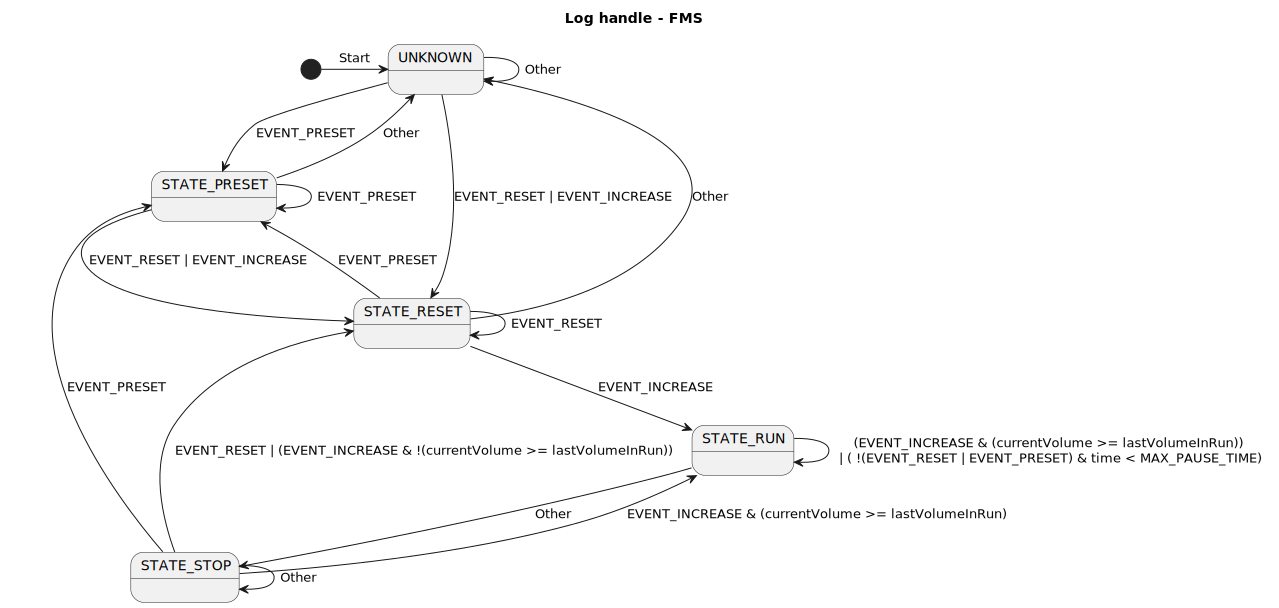
\includegraphics[width=1.0\linewidth]{Figures/LogProcess_Detect-machine-state.png}
    \caption{Sơ đồ trạng thái cho cột bơm}
    \label{fig:LogProcess_Detect-machine-state}
\end{figure}

Sau khi xác định trạng thái mới, hàm callback tương ứng được gọi để kiểm tra phiên bơm mới nếu có:


\begin{longtable}{|c|c|p{3cm}|p{6cm}|}
\hline
\textbf{Trạng thái cũ} & \textbf{Trạng thái mới} & \textbf{Hàm callback} & \textbf{Mô tả} \\
\hline
\endfirsthead

\hline
\textbf{Trạng thái cũ} & \textbf{Trạng thái mới} & \textbf{Hàm callback} & \textbf{Mô tả} \\
\hline
\endhead

\texttt{STATE\_PRESET} & \texttt{STATE\_PRESET} & Check overtime to cut preset & Kiểm tra xem màn hình ở trạng thái PRESET đã được giữ hơn 5 giây chưa. Nếu có, tạo một log mới cho preset. \\
\hline

\texttt{STATE\_RESET} & \texttt{STATE\_RUN} & Generate new Log & Tạo mới một log trống để bắt đầu ghi nhận dữ liệu màn hình. \\
\hline

\texttt{STATE\_RUN} & \texttt{STATE\_RUN} & Update Log info & Trong khi vẫn ở trạng thái RUN, hệ thống cập nhật thông tin log (ví dụ: thời gian, tiền, lít , đơn giá...). \\
\hline

\texttt{STATE\_RUN} & \texttt{STATE\_STOP} & Cut Log & Khi chuyển từ RUN sang STOP, hệ thống chốt log hiện tại  \\
\hline

\caption{Callback được gọi sau khi xác định trạng thái mới}
\label{tab:callback-when-machine-state-changed}
\end{longtable}

\FloatBarrier

\begin{figure}[!ht]
     \centering
    \includegraphics[width=1.0\linewidth]{Figures/flowcharts-DeviceService-OTA.png}
    \caption{Thuật toán thực hiện OTA trên Device Service}
    \label{fig:flowcharts-DeviceService-OTA}
\end{figure}


Các firmware file được gửi tới Device Service dạng base64-string, được kiểm tra tính hợp lệ sau đó lưu vào bộ nhớ tạm.

Khi có yêu cầu kích hoạt firmware, Device Service tiến hành:

\begin{itemize}
    \item Hỏi Thiết bị đọc màn hình file firmware cần cập nhật
    \item Chia file firmware được chọn dưới dạng các chunk độ dài 1000-byte 
    \item Gửi từng chunk tới Thiết bị đọc ghi màn hình cùng offset.
\end{itemize}


\FloatBarrier
\textbf{Thuật toán thực hiện OTA}

\textbf{API cho Client để giao tiếp với Device Service }

Device Service cung cấp API mở để bên Client UI hoặc các bên Client khác có thể giao tiếp để:

\begin{itemize}
    \item Nhận dữ liệu thời gian thực và các phiên bơm (log), trạng thái relay
    \item Yêu cầu cập nhật relay hoặc thực hiện OTA.
\end{itemize}

Dạng dữ liệu: JSON.

Giao thức: TCP.

Mỗi request message là 1 JSON bao gồm các trường

\begin{itemize}
    \item Message ID: UUID định danh message 
    \item Message Type: Loại message để phân loại nội dung.
    \item Và các trường khác là payload tùy thuộc vào Message Type.
\end{itemize}

Các Message Type được hỗ trợ:

\begin{longtable}{|c|p{11cm}|}
\hline
\textbf{MSG Type} & \textbf{Mô tả} \\
\hline
\endfirsthead

\hline
\textbf{MSG Type} & \textbf{Mô tả} \\
\hline
\endhead

0 & Báo cáo sự kiện Log/SubLog từ Device Service tới UI Client. Bao gồm thông tin log hoặc sublog được chốt trong quá trình sử dụng thiết bị. \\
\hline

1 & Báo cáo sự kiện đặt Preset từ Device Service tới UI Client. Được gửi khi nội dung preset không đổi trong 5s hoặc khi chuyển từ preset về reset. \\
\hline

2 & Yêu cầu từ UI Client tới Device Service để thay đổi trạng thái bật/tắt Relay và điều kiện tự động tắt Relay. \\
\hline

3 & Device Service báo cáo trạng thái của các Relay về UI Client. Có thể là phản hồi cho yêu cầu Set Relay hoặc báo cáo chủ động khi có thay đổi. \\
\hline

5 & UI Client gửi yêu cầu tải xuống file firmware về Device Service. File dưới dạng base64, chứa nội dung cần cập nhật cho thiết bị. \\
\hline

6 & UI Client yêu cầu Device Service kích hoạt firmware mới đã được tải xuống. Sau khi thực hiện, thiết bị sẽ tự động reset. \\
\hline

7 & UI Client yêu cầu Device Service trả về danh sách trạng thái hiện tại của tất cả các thiết bị đang quản lý. \\
\hline

8 & Device Service chủ động báo cáo trạng thái của một thiết bị đọc ghi màn hình (kết nối, loại thiết bị, phiên bản firmware...) về cho UI Client. \\
\hline

\caption{Danh sách các message\_type của Device Service}
\label{tab:message-types}
\end{longtable}

\FloatBarrier


Tạo các file log để quan sát tiến trình chạy (hình \ref{fig:logs-txt-files-when-start-DeviceService}):

\begin{itemize}
    \item \texttt{deviceInterface.txt}: file log cho khối Device Interface, ghi các thiết bị đã kết nối, kèm thông báo và lỗi trong quá trình chạy.
    \item \texttt{server-debug.txt}: file log thông báo và lỗi trong quá trình kết nối và giao tiếp Client UI.
    \item \texttt{UDPReport.txt}: Thông báo hiện trạng của tiến trình broadcast UDP.
\end{itemize}

\begin{figure}[!ht]
     \centering
    \includegraphics[width=1.0\linewidth]{Figures/logs-txt-files-when-start-DeviceService.png}
    \caption{Device Service: Các file logs}
    \label{fig:logs-txt-files-when-start-DeviceService}
\end{figure}
\FloatBarrier



% ======================== UI CLIENT ============





\subsubsection{Viết phần mềm Client UI hiển thị các phiên bơm}



\begin{itemize}
    \item Môi trường sử dụng: NodeJS v20.18.1
    \item Ngôn ngữ: TypeScript 
    \item Database: SQLite 
    \item Các thư viện chính sử dụng: ReactJS, sqlite3, MUI Components
\end{itemize}

Các bước triển khai:

Bước 1: Tạo cấu trúc dự án Electron

\begin{itemize}
    \item Sử dụng câu lệnh \texttt{npm create electron-vite@latest} để setup dự án.
    \item Chọn template là ReactJS, ngôn ngữ TypeScript, nhấn \texttt{enter} để bắt đầu tạo mẫu.
\end{itemize}



\begin{figure}[!ht]
     \centering
    \includegraphics[width=1.0\linewidth]{Figures/ElectronViteReact-template.png}
    \caption{Mẫu dự án sử dụng Electron + Vite + ReactJS}
    \label{fig:ElectronViteReact-template}
\end{figure}

\FloatBarrier

Bước 2: Triển khai các tác vụ ở Main Process bao gồm:

\begin{itemize}
    \item Tạo 2 TCP Client:
    \begin{itemize}
        \item Realtime Screen Device Service Client: để nghe dữ liệu màn hình thời gian thực, chuyển tiếp màn hình tới Render Process ở cổng 5001
        \item Event Device Service Client: để nhận phiên bơm (log), điều khiển relay ở cổng 5002. Các phiên bơm nhận được sẽ được chuyển tiếp tới Database ORM.
    \end{itemize}
    \item Tạo Database ORM để đọc ghi cơ sở dữ liệu phiên bơm.
\end{itemize}

Cơ sở dữ liệu phiên bơm gồm 1 bảng lưu các log/sublog gồm các trường:

\begin{figure}[!ht]
     \centering
    \includegraphics[width=0.4\linewidth]{Figures/DeviceService_log-info-entity.png}
    \caption{Các trường lưu trong bảng Log của Database}
    \label{fig:Database_log-info-entity}
\end{figure}

\FloatBarrier

Bước 3: Triển khai giao diện tại Renderer Process

Sử dụng MUI để xây dựng các component:

\begin{itemize}
    \item Khung hiển thị màn hình thiết bị (3 dòng).

    \item Bảng thống kê log/sublog theo thời gian thực.

    \item Lọc, tìm kiếm theo \texttt{device\_id}, \texttt{log\_id}, thời gian, trạng thái, ...

    \item Hiển thị trạng thái kết nối và relay theo từng thiết bị. Các nút điều khiển relay
\end{itemize}

\textbf{Giao diện hoàn chỉnh}
\begin{figure}[!ht]
     \centering
    \includegraphics[width=1\linewidth]{Figures/DeviceServiceClient-init-ui.png}
    \caption{Giao diện hiển thị Client UI}
    \label{fig:DeviceServiceClient-init-ui}
\end{figure}

 